\documentclass[12pt]{article}
\usepackage[utf8]{inputenc}
\usepackage{multicol}
\usepackage{graphicx}
\usepackage{amsmath}
\usepackage{amsfonts}
\usepackage{mathtools}
\usepackage{siunitx}
\usepackage{braket}
\usepackage{parskip}
\usepackage{wrapfig}
\usepackage{xparse,mathtools}

\usepackage[letterpaper, portrait, margin=1in]{geometry}
\renewcommand{\baselinestretch}{1.05}
\title{Quantum HW8}
\author{bellenchia}
\date{March 2019}
\begin{document}
\maketitle

\section*{27.) Spin Precession}
We're given a proton in a magnetic field $B_0$ oriented in the $\hat{z}$ direction, such that after a quarter wave pulse the wavefunction at $t=0$;\\
\begin{center}
$\ket{\Psi(t=0)}=\frac{1}{\sqrt{2}}(\ket{\uparrow}+\ket{\downarrow})$\\
\end{center}

\textbf{a)} To write the Hamiltonian in terms of the Nuclear spin angular momentum operator;\\
(Griffiths deals entirely with \textbf{S} instead of \textbf{I}, I'm making the assumption $S= I$, please don't penalize me for letting the inaccuracy propagating through the whole solution)\\

We know that the energy associated with this torque is $\hat{H}=-\vec{\mu}\cdot\vec{B}$ \\
Also, for a spinning charged particle at rest; $\vec{\mu}=-\gamma\vec{\hat{I}}$\\

Thus, our Hamiltonian is $\hat{H}=-\gamma \vec{\hat{I}}\cdot(B_0\hat{z})=\gamma  B_0\hat{I}_z$\\

\textbf{b)} Now, employing Spinor notation, $\chi=\chi_++\chi_-$ where $\chi_+=\ket{\uparrow}$ and $\chi_-=\ket{\downarrow}$

The Schoedinger equation becomes $\hat{H}\chi=i \frac{d\chi}{dt}$, since we know that\\
\[
\hat{H}\ket{\chi_\pm}=
\begin{cases}
\chi_+ & E_+=-(\gamma B_0 )/2\\
\chi_- & E_-=(\gamma B_0 )/2
\end{cases}
\]

Thus, the wavefunciton times our temporal component is   $\chi(t)=\frac{1}{\sqrt{2}}(e^{i\gamma B_0t/2}\chi_++e^{-i\gamma B_0t/2}\chi_-)$\\
\textbf{c)} To find $\braket{\vec{\hat{I}}}=\sum_{i\in\{x,y,z\}}\braket{\hat{I}_i}\hat{e}_i$ we use the following Pauli matrices,\\

$S_x =  \frac\hbar2\begin{pmatrix} 0 & 1\\1 & 0 \end{pmatrix}$, $S_y =   \frac\hbar2\begin{pmatrix} 0 & -i\\i & 0 \end{pmatrix}$, $S_z =  \frac\hbar2\begin{pmatrix} 1 & 0\\0 & -1 \end{pmatrix}$. To simplify the work, let $i\gamma B_0/2$
%\braket{\chi^\dagger | I_x \chi}=\vect{e^{-\omega},

\section*{28) Nuclear Spin Statistics}
\textbf{a)} The nucleus has spin 1 so that makes it a boson (fermions have half integer spins)\\
\textbf{b)} Allowed energies of I are determined by $|I_1-I_2|\leq I \leq|I_1+I_2|$, since $I_1,I_2$ only take on values 1, 0, -1, we know $I\in\{0,1,2\}$\\

The degeneracy of each I is given by the formula $2i+1$, for example, if $I=2$ then the allowed magnetic sub levels are $-2,1,0,1,2$. All of them are given here;\\
\[
\begin{cases}
I=2 & \rightarrow(2*2+1)=5 different m_I values\\
I=1 & \rightarrow(2*1+1)=3 different m_I values\\
I=0 & \rightarrow(2*0+1)=1 different m_I values\\
\end{cases}
\]
Adding all these together, we see that we have a total number of 9 states. 
\textbf{d) } Clebsch-Gordan time;\\
$I=2$\\
$\ket{2 2}=\ket{1,1}\ket{1,1}$\\
$\ket{2,1}=\frac{1}{\sqrt{2}}\ket{1,1}\ket{1,0}+\frac{1}{\sqrt2}\ket{1,0}\ket{1,1}$\\
$\ket{2,0}=\frac{1}{\sqrt{6}}\ket{1,1}\ket{1,-1}+\sqrt{\frac{2}{3}}\ket{1,0}\ket{1,0}+\frac{1}{\sqrt{6}}\ket{1,-1}\ket{1,1}$\\
$\ket{2,-1}=\frac{1}{\sqrt{2}}\ket{1,0}\ket{1,-1}+\frac{1}{\sqrt{2}}\ket{1,-2}\ket{1,0}$\\
$\ket{2,-2}=\ket{1,-1}\ket{1,-1}$\\
$I=1$\\
$\ket{1,1}=\frac{1}{\sqrt{2}}\ket{1,1}\ket{1,0}-\frac{1}{\sqrt{2}}\ket{1,0}\ket{1,1}$\\
$\ket{1,0}=\frac{1}{\sqrt{2}}\ket{1,11}\ket{1,1}-\frac{1}{\sqrt{2}}\ket{1,1}\ket{1,-1}$\\
$\ket{1,-1}=\frac{1}{\sqrt{2}}\ket{1,0}\ket{1,-1}-\frac{1}{\sqrt{2}}\ket{1,-1}\ket{1,0}$\\
$I=0$\\
$\ket{0,0}=\frac{1}{\sqrt{3}}\ket{1,1}\ket{1,-1}-\frac{1}{\sqrt{3}}\ket{1,0}\ket{1,0}+\frac{1}{\sqrt{2}}\ket{1,-1}\ket{1,-1}$\\
\textbf{e)}  (We assume symmetry refers to the symmetry of exchange between the two nuclei of our diatomic molecule.)\\

When the total \textbf{I} value is even, or zero, we notice that replacing $\ket{I_1}$ with $\ket{I_2}$ yields the same result. For example;\\
$\ket{2,1}=\frac{1}{\sqrt{2}}\ket{1,1}\ket{1,0}+\frac{1}{\sqrt2}\ket{1,0}\ket{1,1}$\\
Swapping $\ket{1,1}$ and $\ket{1,0}$ in place of each other effectively does nothing, this is the same for I=0.\\

For I=1, we see that \\

$\ket{1,0}=-\frac{1}{\sqrt{2}}\ket{1,1}\ket{1,-1}+\frac{1}{\sqrt{2}}\ket{1,-1}\ket{1,1}=-\ket{1,0}$\\

This means our even and odd states are "symmetric" and "antisymmetric," respectively.\\

\textbf{f) } To determine the symmetries allowed for $^{14}N_2$, consider; \\
$\ket{\psi}_{N}=\ket{\psi_{\text{electronic}}}\ket{\psi_{\text{rotational}}}\ket{\psi_{\text{nuclear}}}\ket{\psi_{\text{vibrational}}}$\\



$\ket{\psi}_{N}$ must be symmetric since the nuclei are bosons. This means there must (zero, or) and even number of antisymmetric wavefunctions composing $\ket{\psi}_{{N}}$. We're told the electronic component is symmetric, and vibrations are symmetric by nature, this means we have;\\ $\ket{\psi_{\text{rotational}}}\ket{\psi_{\text{nuclear}}}$ must be symmetric.\\

The value of $I$ determines the symmetry of the nuclear spin wavefunction, for example;\\
When $I$ is odd, the state is antisymmetric. When $\ket{I,m_I}$ is antisymmetric, to ensure the required symmetry of our entire wavefunction, $\ket{\psi_{\text{rotational}}}$ must be antisymmetric. Only allowing antisymmetric rotations, such as spinning about their center of mass. When $I$ is even, the state can describe either nuclei equivalently, this symmetry implies we can only allow an antisymmetric rotation wavefunction, such as spinning about the center of the diatomic molecule.  \\

\textbf{g} When I is odd, we must have the Spherical Harmonic wavefunction $Y^m_J$ be an even function, therefore the state is symmetric, and this happens when I=1 only, so its \textbf{degeneracy} is 1. However, when I=0 or I=2 we are required to have $Y^m_J$ be an odd function/ antisymmetric rotation. So there are two rotational states, one at I=0 and another for I=2, its \textbf{degeneracy} is 2.\\

\textbf{g)} Qualitatively, molecules bounce around quite frequently, it would be incredibly likely to have antisymmetric rotation, an obvious result of random collisions. The only symmetric rotation for a diatomic molecule is about the axis passing through both nuclei.\\

However, a more concrete way of determining this was made clear to me.\\

The number of states where $J=0$ is given by $2J+1=1$ and 
\pagebreak


\section*{29) The Pauli Exclusion Principle}
\textbf{a)}We have $\Psi_e=\frac{1}{\sqrt{2}}[\phi_{1\alpha}(x_1)\phi_{1\alpha}(x_2)-\phi_{1\alpha}(x_1)\phi_{1\alpha}(x_2)]$

We have $\hat{H}=\nabla_1^2+\nabla_1^2+V(r_1,r_2)$\\
$\hat{H}\Psi_e=\frac{1}{\sqrt{2}}\nabla_1^2[\phi_{1\alpha}(x_1)\phi_{1\alpha}(x_2)-\phi_{1\alpha}(x_1)\phi_{1\alpha}(x_2)]+\nabla_1^2[\phi_{1\alpha}(x_1)\phi_{1\alpha}(x_2)-\phi_{1\alpha}(x_1)\phi_{1\alpha}(x_2)]=\frac{10\pi^2}{\sqrt{2}}[sin\pi x_2 sin2\pi x_1-sin\pi x_1sin2\pi x_2]$\\
This implies satisfies the Schroedinger equation, and yields $E=-\frac{10\pi^2}{\sqrt{2}}$\\

\textbf{ b) }

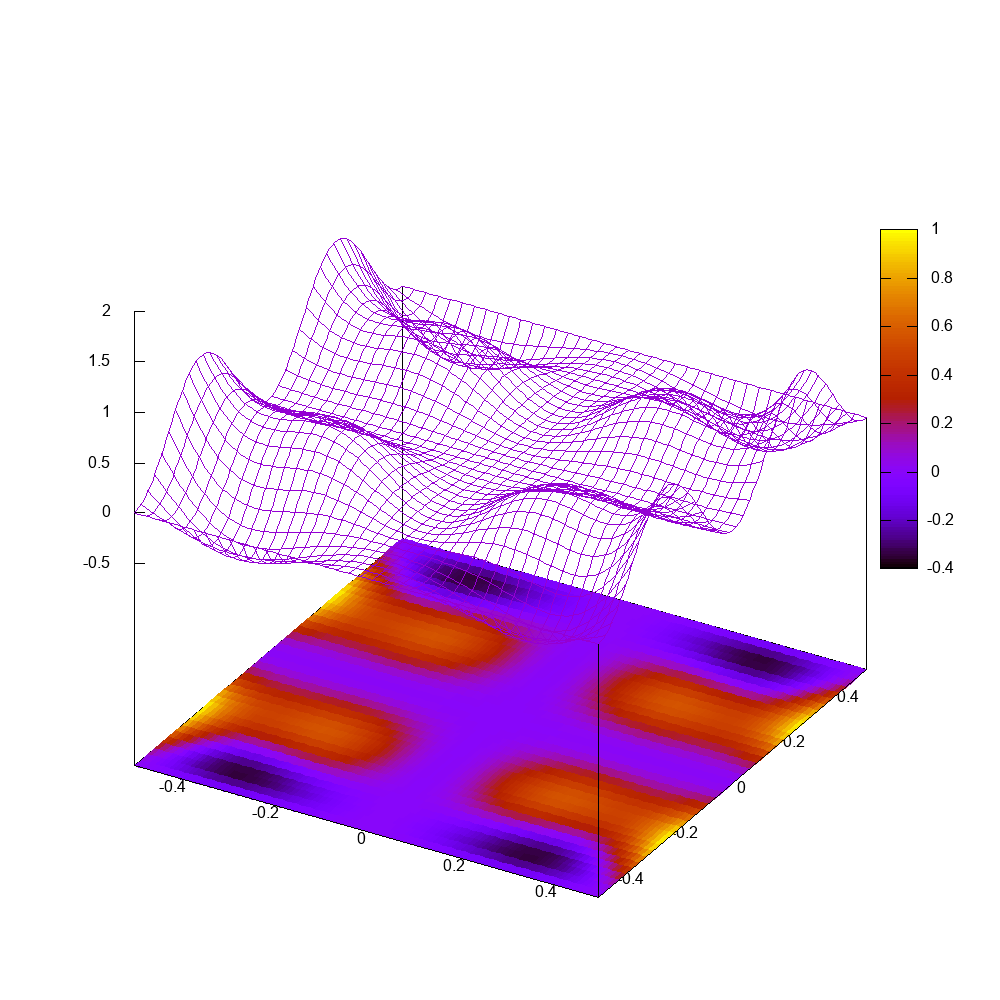
\includegraphics[width=0.8\linewidth]{12.png}

The exclusion principle states that $x_1=x_2\Rightarrow\ket{\Psi}^2\=0$, or that bo 



\end{document}